\documentclass[a4paper,11pt]{book}
\usepackage[utf8]{inputenc}
\usepackage[T1]{fontenc}
\usepackage[english]{babel}
\usepackage{libertinus}
\usepackage{xcolor}
\usepackage{amsmath,amssymb}
\usepackage{graphicx}
\usepackage{booktabs}
\usepackage{tikz}
\usetikzlibrary{arrows.meta,calc}
\usepackage{texweb}

\definecolor{Accent}{HTML}{0B3A3E}
\definecolor{ObsColor}{HTML}{9C5A12}
\definecolor{FigColor}{HTML}{6B3F73}
\definecolor{LemmaColor}{HTML}{4E7A3A}

\numberwithin{equation}{chapter}
\newcommand{\R}{\mathbb{R}}

% a grid of numbers: \numgrid[style]{(x,y)}{cell size}{{row 1},{row 2},...}
\newcommand{\numgrid}[4][]{%
  \edef\numgridlist{#4}%
  \foreach \row [count=\ri] in \numgridlist {%
    \foreach \val [count=\ci] in \row {%
      \node[draw=black!60, minimum size=#3cm, inner sep=0pt, font=\scriptsize, anchor=north west, #1]
        at ($#2 + ({(\ci-1)*#3},{-(\ri-1)*#3})$) {$\val$};
    }%
  }%
}
% a rectangle over a block of cells: \cellrect[style]{(x,y)}{cell size}{col}{row}{n cols}{n rows}
\newcommand{\cellrect}[7][]{%
  \draw[#1] ($#2 + ({#4*#3},{-#5*#3})$) rectangle ++({#6*#3},{-#7*#3});%
}

\usepackage[skins]{tcolorbox}
\newtcolorbox[auto counter, number within=chapter]{definition}[1][]{
  enhanced, frame hidden, sharp corners, colback=Accent!6, coltitle=Accent,
  borderline west={2.5pt}{0pt}{Accent}, fonttitle=\sffamily\bfseries\small,
  attach title to upper={\ }, title={Definition~\thetcbcounter\ifx&#1&\else\ (#1)\fi.}}
\newtcolorbox{remark}[1][]{
  enhanced, frame hidden, sharp corners, colback=ObsColor!8, coltitle=ObsColor,
  borderline west={2.5pt}{0pt}{ObsColor}, fonttitle=\sffamily\bfseries\small,
  attach title to upper={\ }, title={Remark\ifx&#1&\else\ (#1)\fi.}}

\usepackage[backend=bibtex]{biblatex}
\addbibresource{refs.bib}
\usepackage[hidelinks]{hyperref}

\title{texweb example notes}
\author{Emanuele Galiano}

\begin{document}
\maketitle
\tableofcontents

\chapter{How texweb works}\label{ch:intro}
These notes are written in \LaTeX{}, as usual: the same source produces the PDF with \texttt{pdflatex} and the website with \texttt{texweb dev}. References, citations and numbering work in both; for example, chapter~\ref{ch:conv} is about convolution and cites \cite{Goodfellow-et-al-2016}.

\section{What you can write}
The dialect covers everyday commands: \textbf{bold}, \emph{italics}, \texttt{code}, footnotes\footnote{Like this one, numbered per page.} and formulas such as $f(x) = \max\{0, x\}$ or
\begin{equation}\label{eq:loss}
  \mathcal{L}(\vartheta) = \frac{1}{N}\sum_{i=1}^{N} \big(y^{(i)} - h(x^{(i)}; \vartheta)\big)^2, \qquad \vartheta \in \R^d.
\end{equation}
Equation~\eqref{eq:loss} is the MSE.

\begin{definition}[Loss function]\label{def:loss}
A \textbf{loss function} measures the error the model makes when predicting $y$ from $x$.
\end{definition}

Definition~\ref{def:loss} is numbered within the chapter, as in the PDF.

\begin{itemize}
  \item bulleted lists,
  \item numbered lists and tables,
  \item TikZ figures, compiled by \LaTeX{} into SVG.
\end{itemize}

\begin{table}[htbp]
\centering
\begin{tabular}{@{}lrr@{}}
\toprule
Model & Parameters & Layers \\
\midrule
MLP & 397\,510 & 2 \\
CNN & 156 & 1 \\
\bottomrule
\end{tabular}
\caption{Parameters of the first layer on MNIST.}
\label{tab:param}
\end{table}

Table~\ref{tab:param} shows how many parameters are saved.

\chapter{Convolution}\label{ch:conv}
\section{Cross-correlation}
Let $F$ be the input image and $h$ a kernel of size $(2k+1) \times (2k+1)$. The \textbf{cross-correlation} is defined as:
\[
G[i, j] = \sum_{u=-k}^{k}\sum_{v=-k}^{k} h[u, v]\, F[i + u, j + v].
\]

\begin{remark}
What CNNs call convolution is almost always a cross-correlation \cite[ch.~9]{Goodfellow-et-al-2016}.
\end{remark}

\paragraph{Example.}
We apply the \emph{sharpening} kernel to the $5 \times 5$ image of figure~\ref{fig:sharpen}. The jump between the two regions, from 2 to 8 in the input, becomes a jump from $-4$ to 14 in the output: the kernel enhances edges.

\begin{figure}[htbp]
\centering
\begin{widget}{sharpen}[input={{2,2,2,8,8},{2,2,2,8,8},{2,2,2,8,8},{2,2,8,8,8},{2,2,8,8,8}}, kernel={{0,-1,0},{-1,5,-1},{0,-1,0}}, interval=1100]
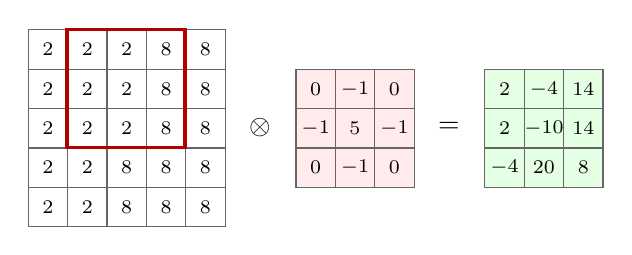
\begin{tikzpicture}
  \numgrid{(0,0)}{0.5}{{2,2,2,8,8},{2,2,2,8,8},{2,2,2,8,8},{2,2,8,8,8},{2,2,8,8,8}}
  \cellrect[very thick, red!70!black]{(0,0)}{0.5}{1}{0}{3}{3}
  \node at (2.95,-1.25) {$\otimes$};
  \numgrid[fill=red!8]{(3.4,-0.5)}{0.5}{{0,-1,0},{-1,5,-1},{0,-1,0}}
  \node at (5.35,-1.25) {$=$};
  \numgrid[fill=green!10]{(5.8,-0.5)}{0.5}{{2,-4,14},{2,-10,14},{-4,20,8}}
\end{tikzpicture}
\end{widget}
\caption{The sharpening kernel applied to a $5 \times 5$ image. The PDF shows the static figure; on the website the kernel slides one position at a time.}
\label{fig:sharpen}
\end{figure}

\section{Padding and stride}
The output size of a convolutional layer is
\[
\text{output} = \frac{W - F + 2P}{S} + 1,
\]
where $W$ is the input side, $F$ the kernel side, $P$ the padding and $S$ the stride \cite{Dumoulin2016}. In figure~\ref{fig:params} you can change all the parameters.

\begin{figure}[htbp]
\centering
\begin{widget}{conv-params}[W=7, F=3, S=2, presets]
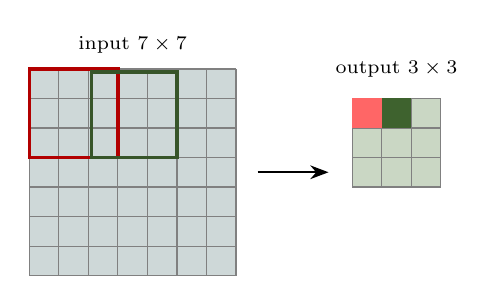
\begin{tikzpicture}[>=Stealth]
  % 7x7 input, 3x3 kernel in two positions with stride 2, 3x3 output
  \fill[Accent!20] (0,0) rectangle (2.625,-2.625);
  \draw[step=0.375, black!50] (0,0) grid (2.625,-2.625);
  \draw[very thick, red!70!black] (0,0) rectangle (1.125,-1.125);
  \draw[very thick, LemmaColor!70!black] (0.79,-0.04) rectangle (1.875,-1.125);
  \draw[->, thick] (2.9,-1.3125) -- (3.8,-1.3125);
  \fill[LemmaColor!30] (4.1,-0.375) rectangle (5.225,-1.5);
  \draw[step=0.375, black!50, shift={(4.1,-0.375)}] (0,0) grid (1.125,-1.125);
  \fill[red!60] (4.1,-0.375) rectangle ++(0.375,-0.375);
  \fill[LemmaColor!80!black] (4.475,-0.375) rectangle ++(0.375,-0.375);
  \node[font=\scriptsize] at (1.3125,0.3) {input $7 \times 7$};
  \node[font=\scriptsize] at (4.6625,0) {output $3 \times 3$};
\end{tikzpicture}
\end{widget}
\caption{The output size formula, with editable parameters. The PDF shows the static figure, with $W = 7$, $F = 3$ and $S = 2$.}
\label{fig:params}
\end{figure}

\begin{figure}[htbp]
\centering
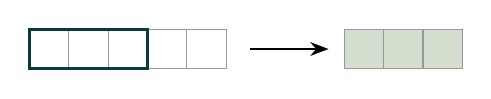
\begin{tikzpicture}[>=Stealth]
  \foreach \i in {0,...,4} \draw[black!40] (\i*0.5,0) rectangle ++(0.5,0.5);
  \draw[very thick, Accent] (0,0) rectangle (1.5,0.5);
  \draw[->, thick] (2.8,0.25) -- (3.8,0.25);
  \foreach \i in {0,...,2} \draw[black!40, fill=LemmaColor!25] (4+\i*0.5,0) rectangle ++(0.5,0.5);
\end{tikzpicture}
\caption{A TikZ figure without a widget: on the website it is the same SVG as in the PDF, compiled from the same preamble.}
\label{fig:static}
\end{figure}


\printbibliography
\end{document}
